\chapter{Concept Realization}\label{cha:concept}

    This section provides the major milestones from the project beginning with a
    brief description of the overall concept solution to the challenges presented
    in the Introduction, followed by the layers of implementation accomplished 
    during the development phase.

%%%%%%%%%%%%%%%%%%%%%%%%%%%%%%%%%%%%%%%%%%%%%%%%%%%%%%%%%%%%%%%%%%%%%%%%%%%%%%%%
%%%%%%%%%%%%%%%%%%%%%%%%%%%%%%%%%%%%%%%%%%%%%%%%%%%%%%%%%%%%%%%%%%%%%%%%%%%%%%%%

\section{Target Scenario}\label{sec:target}

% Goals:
% - open source

% Ideal scenario: 
% - click on a link and run ROS
% - connect to a robot via bluetooth
% - share simulations and algorithms

    To introduce the concept, a ``target scenario'' is first considered. In this
    scenario, an intermediate \ac{ROS} user should be able to reach a high level 
    of usability with the tools developed in this project. First, an
    intermediate user is described as an individual who is familiar with the 
    \ac{ROS} ecosystem but does not have the need to maintain or test \ac{ROS} packages
    across different platforms. In the target scenario, this intermediate
    user will be capable of performing the following tasks:

    \begin{itemize}
        \item install pre-compiled ROS 2 packages in the browser
        \item launch nodes including publishers, subscribers, servers, and clients
        \item interact with the environment to obtain information about 
                running nodes, this would include echoing topics, listing 
                parameters, reviewing log files, etc.
        \item visualize \ac{URDF} files, transforms, point clouds, markers, etc.
        \item play and record bag files % ???
        \item connect with robots via bluetooth
    \end{itemize}

    Outside of this scenario, another goal for this project includes making the 
    developed tools available to the general public by distributing them as
    open-source software. This will allow other roboticists to compile their own
    packages and share them on the web.

%%%%%%%%%%%%%%%%%%%%%%%%%%%%%%%%%%%%%%%%%%%%%%%%%%%%%%%%%%%%%%%%%%%%%%%%%%%%%%%%
%%%%%%%%%%%%%%%%%%%%%%%%%%%%%%%%%%%%%%%%%%%%%%%%%%%%%%%%%%%%%%%%%%%%%%%%%%%%%%%%

\section{Implementation Layers}

    The development of this project is subdivided into multiple levels for the 
    users, the interactions that the users have with the tools developed, and
    the technical difficulty of developing the tools. These subdivisions are
    beneficial in providing the reader with an illustration of the progressing 
    stages of development of this project.


    \begin{tcolorbox}[title=Note]
        \begin{minipage}[t]{0.87\linewidth}
            \vspace*{0pt}
            If the reader would like to follow along with the demonstrations
            provided in the following pages, it is recommended to visit 
            \href{https://ros2wasm.dev/}{\textsf{ros2wasm.dev}}.
            Throughout the text, links will be provided to redirect the reader 
            to specific examples.
        \end{minipage}\hfill%
        \begin{minipage}[t]{0.1\linewidth}
            \vspace*{0pt}
            \includegraphics[height=\linewidth,width=\linewidth]{qr_ros2wasm.png}
        \end{minipage}
    \end{tcolorbox}

%%%%%%%%%%%%%%%%%%%%%%%%%%%%%%%%%%%%%%%%%%%%%%%%%%%%%%%%%%%%%%%%%%%%%%%%%%%%%%%%

    \subsection{User Levels}

        For the purpose of establishing target users for the developed tools,
        potential users were categorized based on expertise level with \ac{ROS} 
        and programming in general. A summary of these levels can be  observed 
        in Table~\ref{tab:userlevels}.

        \begin{table}[htbp]
            \color{textColor}
            \centering	
            \caption{Target users categorized by expertise level.}
                \begin{tabular}{rll}
                    \toprule
                    & \textbf{User}   & \textbf{Description} \\
                    \midrule
                    $1$ & Beginner    & Complete beginners who have never used ROS or programmed \\
                    & & in any language. \\[0.5em]

                    $2$ & Student     & University students with basic programming experience. \\[0.5em]

                    $3$ & ROS User    & Students and researchers who actively use ROS for projects. \\[0.5em]

                    $4$ &  Roboticist & Robotics software developers including contributors to the \\
                    & & ROS ecosystem. \\
                \bottomrule
            \end{tabular}\label{tab:userlevels}
        \end{table}

        Commencing with Level 1, the \textit{Beginner} category is reserved for
        students in secondary education who have had little to no experience with
        programming, and therefore are not familiar with \ac{ROS}. The tools
        developed in this project would serve as an initial introduction to 
        robotics for this category of users.

        Level 2 consists of university students who have completed elementary 
        programming courses but have not yet been introduced to \ac{ROS}. For this
        type of user, this project will provide essential tutorials to become
        acquainted with the inner workings of \ac{ROS}.

        With a slightly higher level of expertise, Level 3 comprises students or
        other enthusiasts who are already familiar with \ac{ROS} and have collaborated
        in projects which use \ac{ROS} as the main system to handle communications
        of multiple robotics elements. This ROS user is equivalent to the intermediate
        user described in the target scenario (Section~\ref{sec:target}).

        Lastly, the highest level of experience is dedicated to roboticists who
        actively use \ac{ROS} and contribute to its development. For this 
        category of users, the intention of this project will be to involve more
        contributors in order to more promptly meet the needs of most \ac{ROS} users.

%%%%%%%%%%%%%%%%%%%%%%%%%%%%%%%%%%%%%%%%%%%%%%%%%%%%%%%%%%%%%%%%%%%%%%%%%%%%%%%%

    \subsection{Interaction Levels}

        The \ac{GUI} is an essential element in the development of this project
        because it determines the benefits the users will receive by utilizing 
        these tools. Similarly, the interface the user experiences with the tools
        has been categorized in increasing levels of interaction. These categories
        are summarized in Table~\ref{tab:uilevels}.

        \begin{table}[htbp]
            \color{textColor}
            \centering	
            \caption{\ac{UI} segmented based on the level of interaction.}
                \begin{tabular}{rll}
                    \toprule
                    & \textbf{Interface} & \textbf{Description} \\
                    \midrule
                    $1$ & Non-interactive & A publisher runs automatically as soon as the site\\
                    & & is loaded. \\ [0.5em]

                    $2$ & Minimal         & User can start/stop a publisher by pressing a button.\\[0.5em]

                    $3$ & Basic           & User can select and run publisher and subscriber \\
                    & & nodes simultaneously.\\[0.5em]

                    $4$ & Intermediate    & Publishers, subscribers, and services are available,\\
                    & & and the user can request basic information about\\
                    & & the environment.\\[0.5em]

                    $5$ & Advanced        & A complete GUI where the user has full control of the \\
                    & & environment, can start/stop nodes, modify parameters, \\
                    & & manage bag files, and visualize robots. \\[0.5em]

                    $6$ & Complete        & All ROS 2 features are available and packages can be \\
                    & & built on the browser, plus the user can directly connect\\
                    & & and interact with external robots.\\

                \bottomrule
            \end{tabular}\label{tab:uilevels}
        \end{table}



        As the name implies, the \textit{non-interactive} Level 1 does not offer the user
        any sort of interaction with the \ac{ROS} environment. With this non-interactive
        interface, the user can do nothing more than load and reload the page. 
        As soon as the user loads the page, a node which has been pre-compiled 
        will automatically start running. In the simplest case scenario, a publisher
        node would run and the published messages would be displayed on the window.
        Because the user has no ability to interact with the environment, this
        publisher node will continue to run uninterrupted. The scenario described
        is illustrated in Figure~\ref{fig:ui1}.

        \begin{figure}[htbp]
            \centering
            % \begin{tikzpicture}
            %     \draw[black, dashed, thin, fill=black!5] (0,0) rectangle (\linewidth,4);
            % \end{tikzpicture}
            \begin{lstlisting}[language=Bash]
Publisher initializing.
[INFO] [168766.57900] [wasm_cpp]: Context initializing.
[INFO] [168767.91500] [wasm_publisher]: Publishing: 'Hello there! 0'
[INFO] [168768.98400] [wasm_publisher]: Publishing: 'Hello there! 1'
[INFO] [168769.94400] [wasm_publisher]: Publishing: 'Hello there! 2'
[INFO] [168770.90300] [wasm_publisher]: Publishing: 'Hello there! 3'
[INFO] [168771.96800] [wasm_publisher]: Publishing: 'Hello there! 4'
[INFO] [168772.92000] [wasm_publisher]: Publishing: 'Hello there! 5'
[INFO] [168773.97600] [wasm_publisher]: Publishing: 'Hello there! 6'
[INFO] [168774.93600] [wasm_publisher]: Publishing: 'Hello there! 7'\end{lstlisting}
            \caption{Output from non-interactive Level 1.}\label{fig:ui1}
        \end{figure}

        \begin{tcolorbox}[title=Example 1]
            \begin{minipage}[t]{0.87\linewidth}
                \vspace*{0pt}
                A demonstration of a \textit{non-interactive} user interface (Level 1) can
                be found at \href{https://ros2wasm.dev/pages/demo01/index.html}{\textsf{ros2wasm.dev/pages/demo01}}

                \textsc{Note:} The page must be reloaded to restart the node.
            \end{minipage}\hfill%
            \begin{minipage}[t]{0.1\linewidth}
                \vspace*{0pt}
                \includegraphics[height=\linewidth,width=\linewidth]{qr_demo01.png}
            \end{minipage}
        \end{tcolorbox}


        By marginally expanding the interface, the \textit{minimal} Level 2 provides
        the user with the ability to start and stop a pre-compiled node. This 
        stage is accomplished by the addition of buttons to the website. Continuing
        with the example previously described, in this level the user can press
        a button to start a publisher node, view the output of any published 
        messages, and stop the node at any point. Level 2 is exhibited in Figure~\ref{fig:ui2}

        \begin{figure}[htbp]
            \centering
            \includegraphics[width=\linewidth]{03_level2.png}
            \begin{lstlisting}[language=Bash]
[INFO] [16879468.55200] [wasm_publisher]: Publishing: 'Hello there! 13'
[INFO] [16879469.60800] [wasm_publisher]: Publishing: 'Hello there! 14'
[INFO] [16879470.56000] [wasm_publisher]: Publishing: 'Hello there! 15'
[INFO] [16879471.61600] [wasm_publisher]: Publishing: 'Hello there! 16'
[INFO] [16879472.56800] [wasm_publisher]: Publishing: 'Hello there! 17'
[INFO] [16879473.62400] [wasm_publisher]: Publishing: 'Hello there! 18'
Publisher terminated.\end{lstlisting}
            \caption{Interactive buttons to start and stop the publisher node.}\label{fig:ui2}
        \end{figure}

        \begin{tcolorbox}[title=Example 2]
            \begin{minipage}[t]{0.87\linewidth}
                \vspace*{0.5\baselineskip}
                A demonstration of a \textit{minimal} user interface (Level 2) can
                be found at \href{https://ros2wasm.dev/pages/demo02/index.html}{\textsf{ros2wasm.dev/pages/demo02}}
            \end{minipage}\hfill%
            \begin{minipage}[t]{0.1\linewidth}
                \vspace*{0pt}
                \includegraphics[height=\linewidth,width=\linewidth]{qr_demo02.png}
            \end{minipage}
        \end{tcolorbox}



        The \textit{basic} Level 3 offers the user increasingly more control over
        the environment. In this level, the user has the ability to run more than
        one node simultaneously. This makes it possible to have publishers sending
        messages to a particular topic and subscribers retrieving the published
        messages accordingly. Nonetheless, the nodes are still pre-compiled and 
        thus the user does not have the ability to change the topic names or any
        other parameters of the nodes. Figure~\ref{fig:ui3} demonstrates a snapshot 
        of Level 3.

        \begin{figure}[htbp]
            \centering
            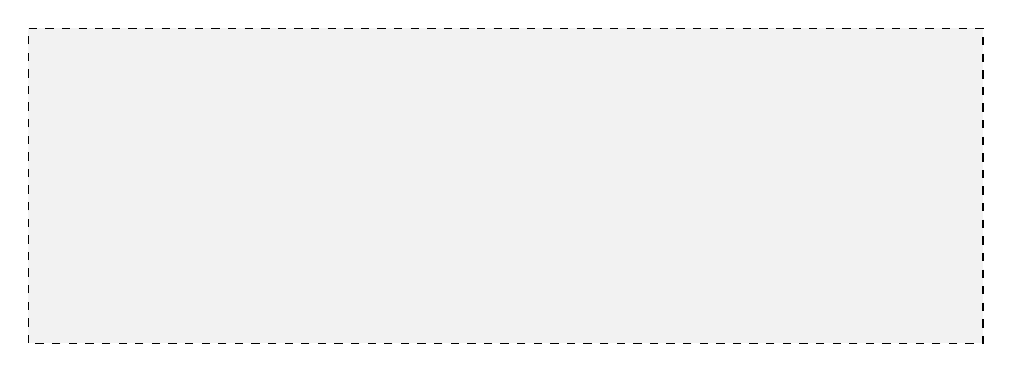
\begin{tikzpicture}
                \draw[black, dashed, thin, fill=black!5] (0,0) rectangle (\linewidth,4);
                \end{tikzpicture}
            \caption{TODO Level 3 image}\label{fig:ui3}
        \end{figure}

        \begin{tcolorbox}[title=Example 3]
            \begin{minipage}[t]{0.87\linewidth}
                \vspace*{0.5\baselineskip}
                A demonstration of a \textit{basic} user interface (Level 3) can
                be found at \href{https://ros2wasm.dev/pages/demo03/index.html}{\textsf{ros2wasm.dev/pages/demo03}}
            \end{minipage}\hfill%
            \begin{minipage}[t]{0.1\linewidth}
                \vspace*{0pt}
                \includegraphics[height=\linewidth,width=\linewidth]{qr_demo03.png}
            \end{minipage}
        \end{tcolorbox}



        Stepping further into the list, the \textit{intermediate} Level 4 introduces
        services, these include both the servers and the clients. Additionally,
        with this level the users now possess the ability to request information
        from the environment such as the type of nodes which are running at a
        given time, or which topics are available. A depiction of Level 4 is shown
        in Figure~\ref{fig:ui4}

        \begin{figure}[htbp]
            \centering
            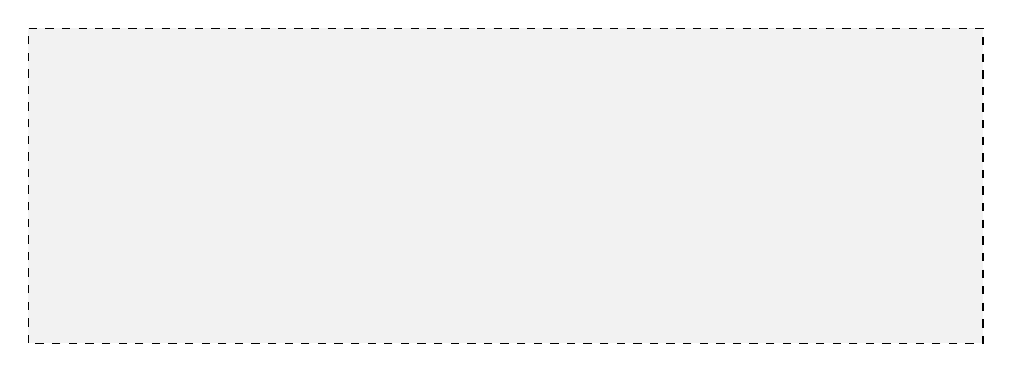
\begin{tikzpicture}
                \draw[black, dashed, thin, fill=black!5] (0,0) rectangle (\linewidth,4);
                \end{tikzpicture}
            \caption{TODO Level 4 image}\label{fig:ui4}
        \end{figure}

        \begin{tcolorbox}[title=Example 4]
            \begin{minipage}[t]{0.87\linewidth}
                \vspace*{0.5\baselineskip}
                A demonstration of an \textit{intermediate} user interface (Level 4) can
                be found at \href{https://ros2wasm.dev/pages/demo04/index.html}{\textsf{ros2wasm.dev/pages/demo04}}
            \end{minipage}\hfill%
            \begin{minipage}[t]{0.1\linewidth}
                \vspace*{0pt}
                \includegraphics[height=\linewidth,width=\linewidth]{qr_demo04.png}
            \end{minipage}
        \end{tcolorbox}



        Finally arriving at the \textit{advanced} Level 5, this level is more 
        prominent because it introduces the integration of JupyterLite with the 
        ROS environment. With JupyterLite, the user can directly interact with
        the ROS environment by using the ROS client libraries such as \texttt{rclpy}.
        A typical workspace in JupyterLite is pictured in Figure~\ref{fig:ui5}.

        \begin{figure}[htbp]
            \centering
            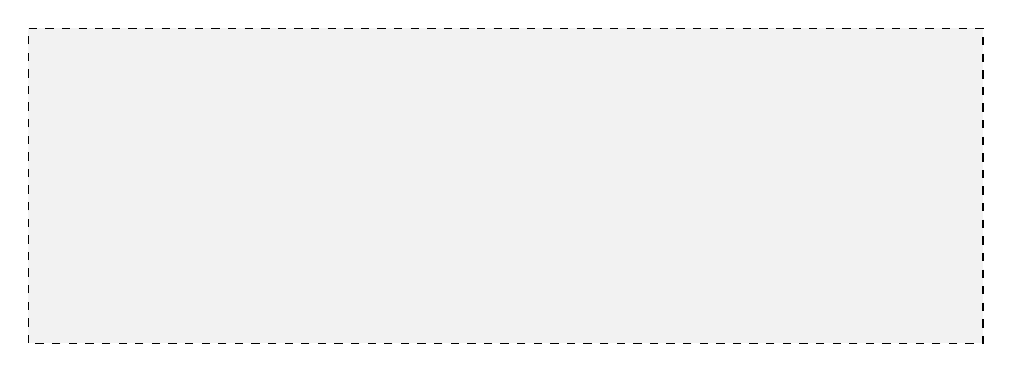
\begin{tikzpicture}
                \draw[black, dashed, thin, fill=black!5] (0,0) rectangle (\linewidth,4);
                \end{tikzpicture}
            \caption{TODO Level 5 image}\label{fig:ui5}
        \end{figure}

        % NO DEMO HERE
        % \begin{tcolorbox}[title=Example 5]
        %     \begin{minipage}[t]{0.87\linewidth}
        %         \vspace*{0.5\baselineskip}
        %         A demonstration of an \textit{advanced} user interface (Level 5) can
        %         be found at \href{https://ros2wasm.dev/pages/demo05/index.html}{\textsf{ros2wasm.dev/pages/demo05}}
        %     \end{minipage}\hfill%
        %     \begin{minipage}[t]{0.1\linewidth}
        %         \vspace*{0pt}
        %         \includegraphics[height=\linewidth,width=\linewidth]{qr_demo05.png}
        %     \end{minipage}
        % \end{tcolorbox}


        Lastly, Level 6 consists of a \textit{complete} ROS environment also made available to the user through JupyterLite. The user would be able to install any additional ROS packages from \texttt{emscripten- forge}. An extension for JupyterLite could enable communications with external robots by using the Web Bluetooth API.\@ And a web compiler could be implemented to directly build packages within JupyterLite.

%%%%%%%%%%%%%%%%%%%%%%%%%%%%%%%%%%%%%%%%%%%%%%%%%%%%%%%%%%%%%%%%%%%%%%%%%%%%%%%%

    \subsection{Complexity Levels}

        In regards to technical complexity of the project, a series of complexity levels is outlined in Table~\ref{tab:techlevels}. The first four levels (1-4) must be accomplished in strict order, while levels 5-8 do not have any dependencies on the preceding levels to be able to function.        

        \begin{table}[htbp]
            \color{textColor}
            \centering	
            \caption{Implementation categories with increasing technical complexity.}
                \begin{tabular}{cl}
                    \toprule
                    \textbf{Level} & \textbf{Description} \\
                    \midrule
                    $1$ & Replacement of the \ac{ROS} middleware implementation. \\ [0.3em]
                    $2$ & A custom package and its dependencies can be cross-compiled to WebAssembly. \\[0.3em]
                    $3$ & A publisher and subscriber can communicate with each other on the browser.\\[0.3em]
                    $4$ & Multiple nodes and distinct topics can run simultaneously. \\[0.3em]
                    $5$ & Manipulation of a physical robot via bluetooth or wifi. \\[0.3em]
                    $6$ & Interaction with a ROS client library from JupyterLite. \\[0.3em]
                    $7$ & Visualization of a robot with Amphion and Zethus. \\[0.3em]
                    $8$ & Simulation of a robotics scenario with Gazebo. \\[0.3em]
                    $9$ & Development workspace for creating and debugging ROS packages. \\
                \bottomrule
            \end{tabular}\label{tab:techlevels}
        \end{table}

        Although creating a replacement for the \ac{ROS} middleware implementation denotes the lowest level on the list, its complexity must not be underestimated. Level 1 consists of creating custom middleware packages to handle discovery and communications between nodes. All other \ac{ROS} packages depend on the middleware implementation, and because of this, creating a working replacement is crucial before any other features can be implemented.

        Once the middleware packages have been introduced, the next level ensures that the core \ac{ROS} packages can be cross-compiled. Level 2 involves the creation of a recipe to build all packages consistently. Minor modifications are needed in a few of the core packages to prevent compilation errors; for details, refer to TODO: add mods to appendix. And in order to set the custom middleware implementation as default, packages belonging to the other implementations must be ignored or removed. 

        Continuing the progression, Level 3 involves cross-compiling a package containing two executables, a publisher and a subscriber. Once these nodes are successfully loaded on the browser, communication between the nodes must be established by passing messages between web workers and the main thread.

        Level 4 is simply an expansion of Level 3. In this case, the system handling communication between nodes can accommodate a multitude of different topics, message types, and node types. In other words, the communication system must be able to create and remove message queues at the time when they are requested by the individual nodes.

        Starting with Level 5, the project begins to develop more practical applications. Manipulating a robot from the browser involves the addition of external libraries which enable communications to the hardware components of the robot. For example, a library which uses the Web Bluetooth \ac{API} to establish a connection to a robot and sends commands commands to activate the robot's motors. This level also involves creating an interface which translates \ac{ROS} messages to commands the robot can receive.

        Level 6 requires Python support on the browser. This step consists of cross-compiling the \ac{ROS} client library for Python (\texttt{rclpy}) in order to be able to import it from JupyterLite. The benefit of importing \texttt{rclpy} is that nodes could be created directly from the browser as shown in Figure~\ref{fig:rclpy}. 

        \begin{figure}[htbp]
            \centering
            \begin{lstlisting}[language=Python]

  import rclpy
  web_node = rclpy.create_node("web_node")
            \end{lstlisting}
            \caption{Example of creating a node with \textsf{rclpy}.}
            \label{fig:rclpy}
        \end{figure}

        Visualization of robots begins with Level 7. For this step, the Amphion and Zethus libraries are adapted to receive information from the \ac{ROS} 2 nodes running on the browser. This entails replacing or modifying the dependency on \texttt{rosjslib} (the \ac{ROS} 1 JavaScript library) which interacts with a native \ac{ROS} 1 environment from the browser. Currently, \texttt{roslibjs} does not actively support \ac{ROS} 2, but this is likely to change in the near future as more systems transition to \ac{ROS} 2.

        Unlike Amphion and Zethus, recent versions of Gazebo do support simulations for \ac{ROS} 2 ecosystems. However, for Level 8, Gazebo's tools and libraries would need to be modified to run on the browser or communications must be established to Gazebo's cloud servers.

        Lastly, Level 9 culminates with the implementation of all the previous levels plus additional developer tools such as compilers and debuggers running on the browser which would be equivalent to developing \ac{ROS} packages in a local machine.
